\PassOptionsToPackage{dvipsnames,table}{xcolor}
\documentclass[10pt]{beamer}
\usepackage{Cours}


\begin{document}

\input{\detokenize{/home/fenarius/Travail/Cours/cpge-info/latex//MacrosCours.tex}}

% Numéro et titre de chapitre
\setcounter{numchap}{4}
\newcommand{\Ctitle}{\cnum $k$ plus proches voisins, $k$ moyennes}

\makess{\textit{knn} : exemple introductif}
\begin{frame}{\Ctitle}{\stitle}
    \begin{exampleblock}{Un champ de fleurs}
        Dans un champ, à l'état sauvage deux types de fleurs ont poussés : des coquelicots et des violettes. On a représenté ci-dessous par un schéma la position de ces fleurs dans le champ
        \begin{center}
            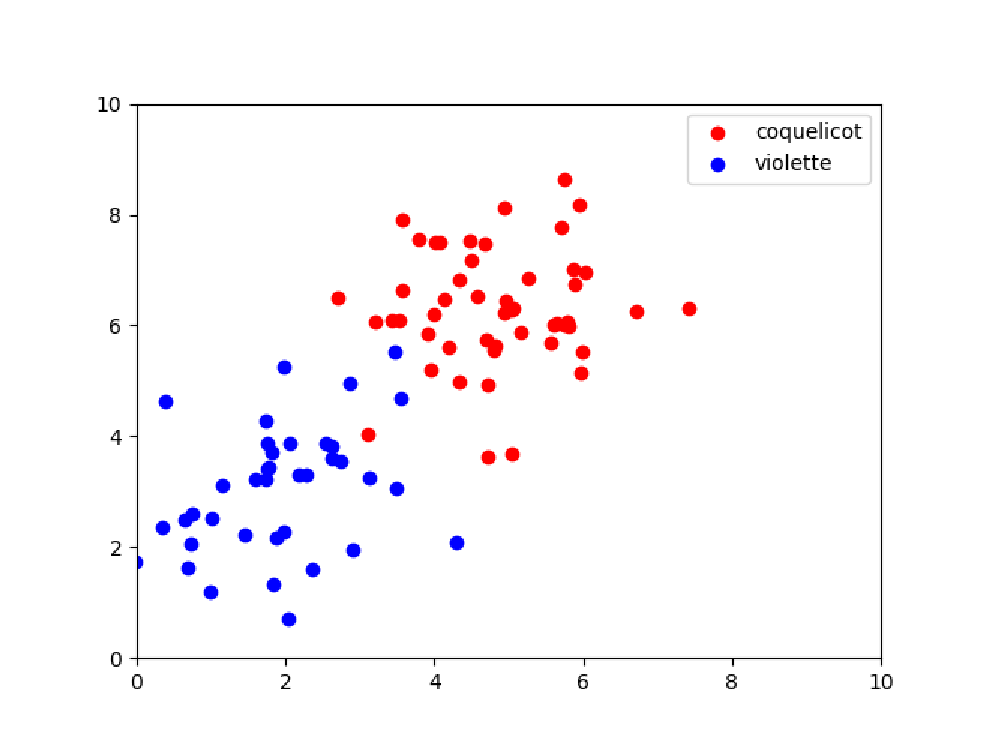
\includegraphics[height=5cm]{ex_cours1.eps}
        \end{center}
    \end{exampleblock}
\end{frame}


\begin{frame}{\Ctitle}{\stitle}
    \begin{exampleblock}{Un champ de fleurs}
        Trois nouvelles pousses, notées $P_1$, $P_2$ et $P_3$ (en gris sur le schéma) font leur apparition. Et on cherche à prédire si ces pousses sont des coquelicots ou des violettes.
        \begin{center}
            \includegraphics[height=5cm]{ex_cours2.eps}
        \end{center}
    \end{exampleblock}
\end{frame}


\begin{frame}{\Ctitle}{\stitle}
    \begin{exampleblock}{Un champ de fleurs}
        On a tracé ci-dessous un cercle de façon apparaître les 5 voisins les plus proches de $P_3$. Choisir l'espèce majoritaire de ce cercle pour classer la nouvelle pousse $P_3$ est un exemple de l'application des $5$ plus proches voisins (\textit{nearest neighbours} en anglais, abrégé en \textit{nn})
        \begin{center}
            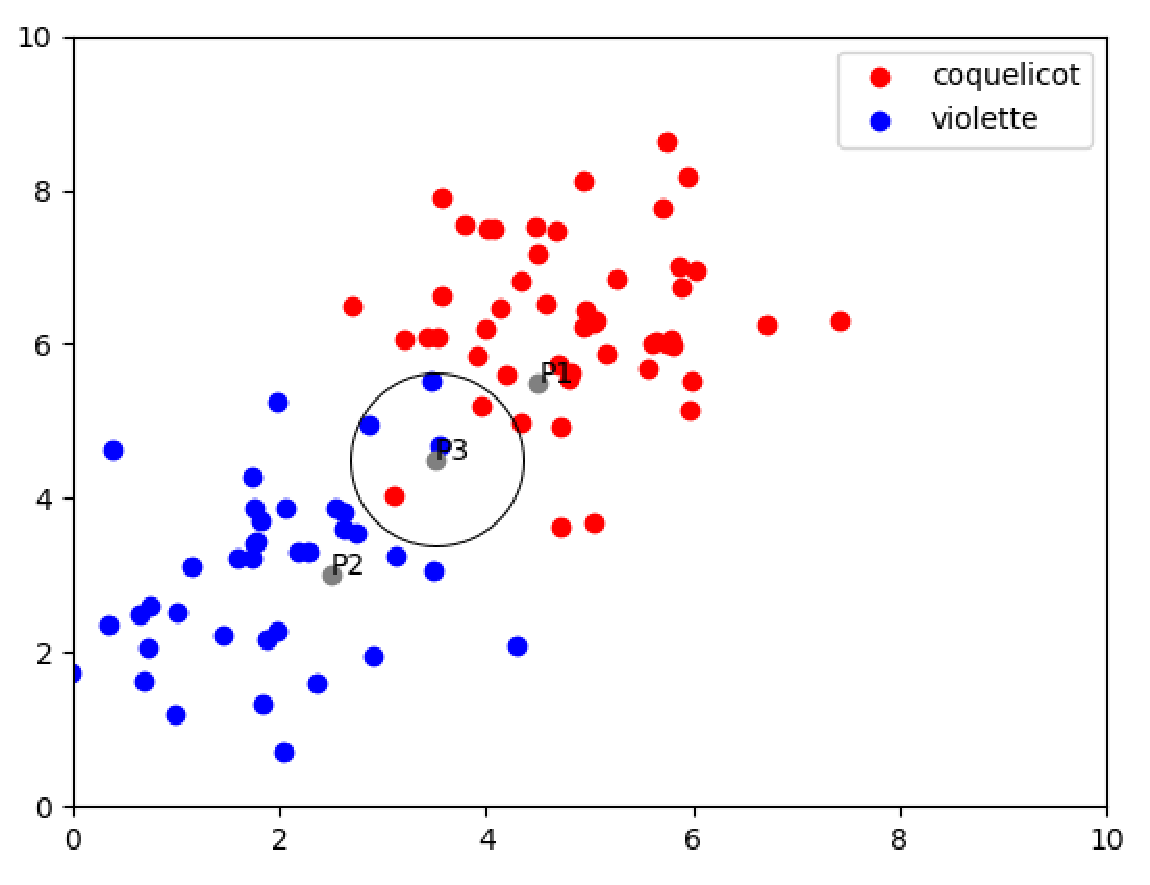
\includegraphics[height=5cm]{ex_cours3.eps}
        \end{center}
    \end{exampleblock}
\end{frame}

\makess{\textit{knn} : principe de l'algorithme}
\begin{frame}{\Ctitle}{\stitle}
	\begin{alertblock}{Principe de l'algorithme}
		\begin{itemize}
			\item<1-> L'algorithme des \textcolor{red}{$k$ plus proches voisins} est un algorithme de classification des données appartenant à la famille des algorithmes d'apprentissage supervisé.
			\item<2-> On dispose d'un jeu de données qui associe chaque donnée à une classe.
			\item<3-> L'algorithme attribut à une nouvelle donnée $d$ non classée la classe majoritaire de ses $k$ plus proches voisins.
			\item<4-> On doit donc utiliser une distance sur l'ensemble des données (par exemple la distance euclidienne)
		\end{itemize}
	\end{alertblock}
\end{frame}


\begin{frame}{\Ctitle}{\stitle}
	\begin{exampleblock}{Exemple}
		\begin{center}
		\includegraphics[scale=0.25]{knn1.eps}
		\end{center}
		Le point gris central est la donnée à classer. Quel sera le résultat de l'algorithme :
		\begin{itemize}
			\item<2->{Pour $k=3$ ?}
			\onslide<4->{\textcolor{OliveGreen}{Il y 2 croix et un losange dans les 3 plus prochains voisins, la classe majoritaire est donc la croix et l'algorithme classe la donnée comme une croix.}}
			\item<3->{Pour $k=10$ ?}
			\onslide<5->{\textcolor{OliveGreen}{Cette fois il y a 6 losanges et 4 croix parmi les 10 plus proches voisins, la donnée est donc classée parmi les losanges.}}
		\end{itemize}
	\end{exampleblock}
\end{frame}


\begin{frame}{\Ctitle}{\stitle}
    \begin{block}{Synthèse}
        La mise en oeuvre de l'algorithme demande donc à :
        \begin{itemize}
            \item<1-> Disposer d'un jeu de données $d=(d_0, \dots d_{n-1})$ déjà classées, c'est à dire attribuées à des classes $c_0, \dots c_{m-1}$
            \item<2-> D'une distance entre deux données de façon à quantifier la notion de proximité.
            \item<3-> Choisir un nombre $k$ de voisins à considérer. La valeur de $k$ influence la prédiction de l'algorithme (voir exemple précédent). En pratique, on teste plusieurs valeurs de $k$ et on choisit celle qui donne les meilleurs résultats.
            \item<4-> Une nouvelle donnée $d_n$ est alors affectée à la classe de ses $k$ plus proches voisins.
        \end{itemize}
    \end{block}
\end{frame}


\makess{\textit{knn} : mise en oeuvre en Python}
\begin{frame}{\Ctitle}{\stitle}
    On suppose qu'on dispose :
    \begin{itemize}
        \item<2-> d'un jeu de données $(d_0, \dots d_{n-1})$
        \item<3-> d'une fonction \kw{distance} prenant en argument deux données $d_1$ et $d_2$ et calculant la distance qui les sépare
        \item<4-> d'une nouvelle donnée $e$ non encore classée
    \end{itemize}
    
\end{frame}

\end{document}